\documentclass{beamer}

\usetheme{uhh}
\showtotalframenumber
\showuhhlogoeachframe
\showsections

\usepackage{amsmath}
\usepackage{graphicx}
\usepackage{color}
\DeclareMathOperator*{\argmin}{arg\,min}

\usepackage{listings}
\lstset{
  language=python
  }


\title{Inducing Interpretable Word Senses for WSD and Enrichment of Lexical Resources}

%\institute[University of Hamburg] 
%{
%  Faculty of Mathematics, Informatics, and Natural Sciences \\
%  Department of Informatics\\
%  Language Technology Group
%}


\author{Alexander Panchenko} % \\University of Hamburg, Germany}
\date[11.02.2018]{Jan 11, 2018}


\AtBeginSection[]
{
   %%%%% section title
   % This is how it would look like in Beamer:
   % \begin{frame}
   %     \frametitle{Overview}
   %     \tableofcontents[sections={2-3},currentsection,sectionstyle=show/hide,subsectionstyle=hide]
   % \end{frame}
  \begin{frame}[plain]
  \begin{tikzpicture}[overlay]
    \relax%
    \fill[blueuhh,opacity=1] (-10,-10)
    rectangle(\the\paperwidth,\the\paperheight);
  \end{tikzpicture}
   \begin{tikzpicture}[overlay]
    \relax%
    \fill[white,opacity=1] (-5,-1.2)
    rectangle(\the\paperwidth,0.5) node[pos=0.5,black]{\LARGE\insertsectionhead};
  \end{tikzpicture}
  \end{frame}

  %%%% add subsection to show navigation dots
  \subsection{}
}

\begin{document}

\maketitle

\begin{frame}
  \frametitle{Overview}

  \begin{itemize}
		\item \textbf{Inducing word sense representations}:
		\begin{itemize}
		\item word sense embeddings via retrofitting \cite{pelevina-EtAl:2016:RepL4NLP,remus:2018};
		\item sparse sense representations \cite{panchenko-EtAl:2017:EACLlong};
		\item sense semantic classes \cite{panchenko:2018:SemanticClasses} 
		\end{itemize}
		
	\pause 
	\vspace{1em}
	\item \textbf{Making the induced senses interpretable} \cite{panchenko-EtAl:2017:EMNLP2017Demos,panchenko-EtAl:2017:EACLlong}
	
	\pause
	\vspace{1em}
	\item \textbf{Linking induced word senses to lexical resources}~\cite{faralli2016linked,panchenko-EtAl:2017:SENSE2017,biemann2018framework}	
			
\end{itemize}
	
\end{frame}

\section{Inducing word sense representations}


\begin{frame}[fragile]
\frametitle{Related work}
\begin{center}
 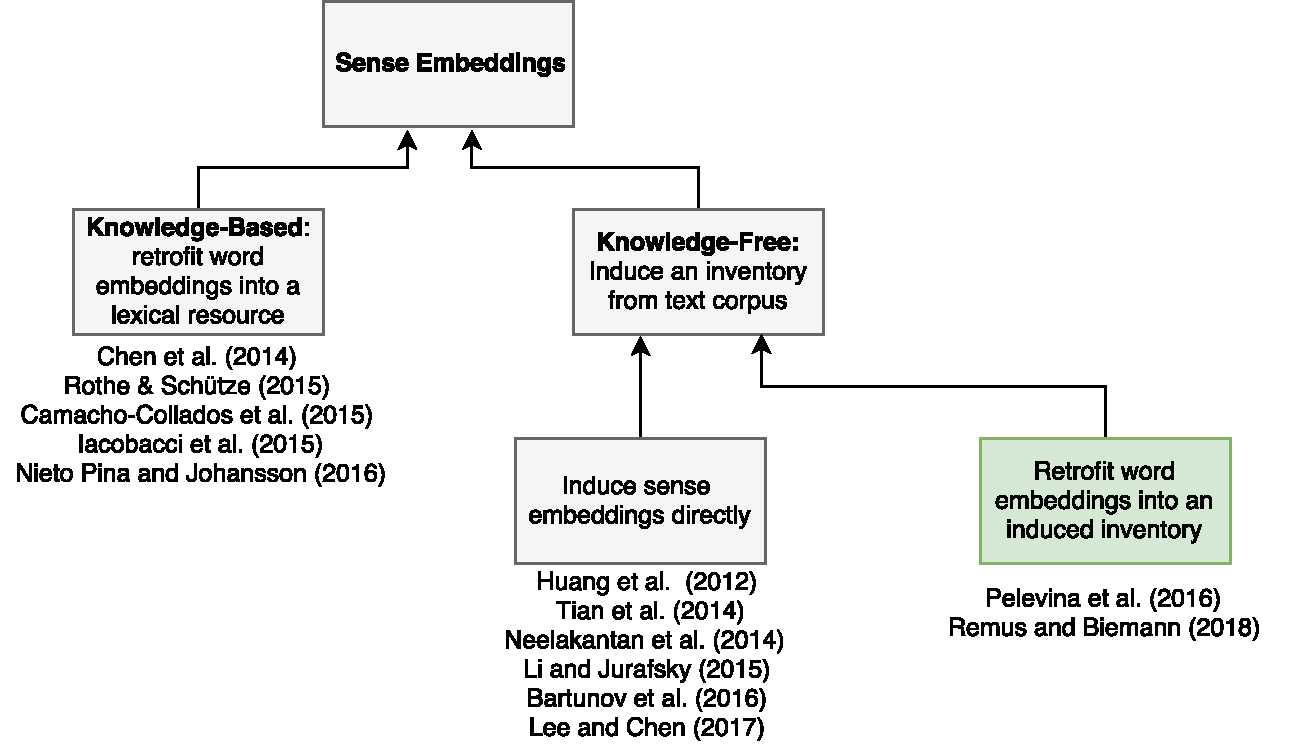
\includegraphics[height=0.56\textwidth]{sense_embeddings}
 \end{center}
\end{frame}


\begin{frame}
\frametitle{Related work: knowledge-based}
\begin{itemize}
	\item \textbf{AutoExtend}~\cite{rothe-schutze:2015:ACL-IJCNLP}
\end{itemize}
\begin{center}
 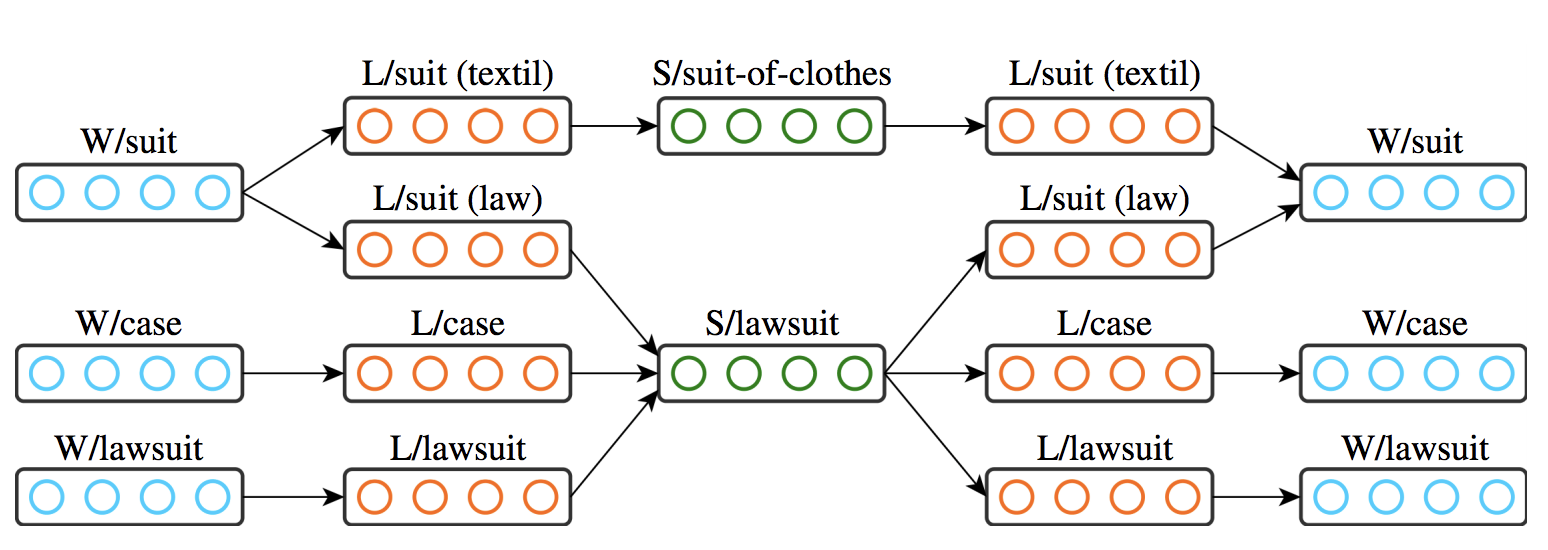
\includegraphics[width=1.0\textwidth]{autoextend}
 \end{center}

{\footnotesize
 * image is reproduced from the original paper
}

\end{frame}

\begin{frame}{Related work: knowledge-free}

\begin{itemize}
\item \textbf{Adagram}~\cite{bartunov2016breaking}
\item Multiple vector representations $\theta$ for each word:
%\item An bayesian extension of the Skip-gram model:
 $$p(Y,Z,\mathbf{\beta}|X,\alpha,\theta) = \prod_{w=1}^{V} \prod_{k=1}^{\infty} p(\beta_{wk}|\alpha) \prod_{i=1}^N [p(z_i|x_i,\mathbf{\beta}) \prod_{j=1}^C p(y_{ij}|z_i,x_i,\theta)],$$ 
\begin{itemize}
\item $\alpha$ -- a meta-parameter controlling number of senses;
\item $z_i$ -- a hidden variable: a sense index in context; 
\item $p(\beta_{wk}|\alpha)$ -- probability of the $k$-th sense of the word $w$;
\item $p(z_i|x_i,\mathbf{\beta})$ -- probability of observing word $x_i$ in the sense $z_i$;
\item $\prod_{j=1}^C p(y_{ij}|z_i,x_i,\theta)$ -- probability of the context $C$.
\end{itemize}

\pause 
\item \alert{\textbf{See also}}: [Neelakantan et al., 2014] and [Li and Jurafsky, 2015]

\end{itemize}
	
\end{frame}




\begin{frame}{Sense embeddings using retrofitting}
	
\end{frame}

\begin{frame}{Sense embeddings using retrofitting}
	
\end{frame}



\begin{frame}{Sparse sense representations}
	
\end{frame}


\begin{frame}{Sparse sense representations}
	
\end{frame}


\begin{frame}{Sparse sense representations}
	
\end{frame}

\begin{frame}{Watset: synset induction}
	
\end{frame}


\begin{frame}{Watset: synset induction}
	
\end{frame}


\begin{frame}{Watset: synset induction}
	
\end{frame}


\begin{frame}{Induction of sense semantic classes}
	
\end{frame}

\begin{frame}{Induction of sense semantic classes}
	
\end{frame}

\begin{frame}{Induction of sense semantic classes}
	
\end{frame}


\section{Conclusion}

\begin{frame}{Summary}

\begin{itemize}
	\item How to \textbf{induce word senses}, \textbf{synsets} and \textbf{semantic classes} from text and synonyms.
    \vspace{1em}
    \pause
    
	\item \textbf{Interpretability can be added} on the top of induced word senses in a model agnostic way. 
	\vspace{1em}
    \pause
	
	\item Hypernymy labels \textbf{improve hypernymy extraction}. 
	\vspace{1em}
	\pause
	
	\item Linking induced word senses to lexical resources:
	\begin{itemize} 
		\item improves \textbf{performance of WSD};
		\item can be used to \textbf{enrich lexical resources} with new senses.
	\end{itemize}
	
	
\end{itemize}


\end{frame}


\begin{frame}{A New Shared Task on WSI\&D}
  
  \begin{itemize}
  \item Participate in an ACL SIGSLAV sponsored shared task on \textbf{word sense induction and disambiguation} for Russian!
  
  
 \end{itemize} 
  
  \begin{block}{A lexical sample task evaluated using the ARI measure }
  \begin{itemize}
  	\item Target word, e.g. ``bank'' (in Russian).
  	\item Contexts where the word occurs.
  	\item You need to group the contexts by senses.
  \end{itemize}
   \end{block}
  
  \pause
  \begin{itemize}
    \item \textbf{More details}: \url{http://russe.nlpub.org/2018/wsi}
  \item You can participate by \textbf{31.01.2018}.
     
  \end{itemize}
  
\end{frame}

\begin{frame}{}
\Huge{Thank you!}
\end{frame}

\bibliography{biblio}
\bibliographystyle{apalike}


\end{document}

